\documentclass[12pt]{article}
\usepackage{cite}
\usepackage{tikz}
\usepackage{float}
\usepackage{tikz-qtree}
\usepackage{pgfplots}

\title{Parse-tree-grams in word embedding.}
\author{Ilya Feldshteyn}

 
\begin{document}
\maketitle

\begin{abstract}
We are introducing parse-tree-grams (PT-grams)
\end{abstract}


\section{Introduction}

Statistical methods of text analysis relay among other
text characteristics on word co-occurrences.
Words systematically found close to each other in texts
allows us to think about a common context. Word
embedding techniques -- word2vec and its modifications --
associate a word with a vector in a multi-dimensional
space and words used together in different texts are
expected to be close in that space.

This approach is easy to implement and scale,
but the view of a text as a flat flow of words has
certain drawbacks. Text has a hierarchical structure
and not all words co-occurrences are equally important.
The problem is not new, some efforts were made to take
into account the issue
(see for example \cite{DBLP:journals/corr/AvrahamG17}).

In this article we consider a modification of
skip-gram that takes into account the hierarchical structure of the
text. Words co-occurrence is considered with respect to a
word position in a parse tree -- words form a parse-tree-gram
(PT-gram) if they belong to the same sub-tree of a parse tree.
Instead of words in a fixed-size window we are first building
a parse tree of a sentence and analyze its structure. This gives
us several variable-size windows for the same part of a sentence
or a sentence as a whole.

To evaluate the effect of using PT-grams we've built
two word2vec embeddings -- using skip-grams and PT-grams representations --
and compared their performance on analogy test
\cite{DBLP:journals/corr/abs-1301-3781}.

\section{Calculations}

For the purposes of this study we were using relatively small
corpus of 1 million sentences from Wikipedia \cite{leipzigcorpora},
Stanford CoreNLP \cite{corenlp} to build parse trees, and
Tensorflow \cite{tensorflow} for word2vec program.

Parse trees split into subtrees form variable-size PT-grams
(see Appendix for examples).
Average size of subtrees is 4.2 words.
This size was used as a reference to construct
window of comparable size (-2,+2) for skip-grams.

Two embeddings (300-dimensional space)
were generated with the same parameters and models were trained
for the same iterations.

\section{Results}

Below are results of the analogy test for skip-gram and PT-gram
models (note that the goal of this study is to compare the effect
of using parse tree structure in word embedding, not to beat the
best models in the field).

\begin{center}
\begin{figure}[H]
\caption{Accuracy test results for skip-grams and PT-grams},
\centering
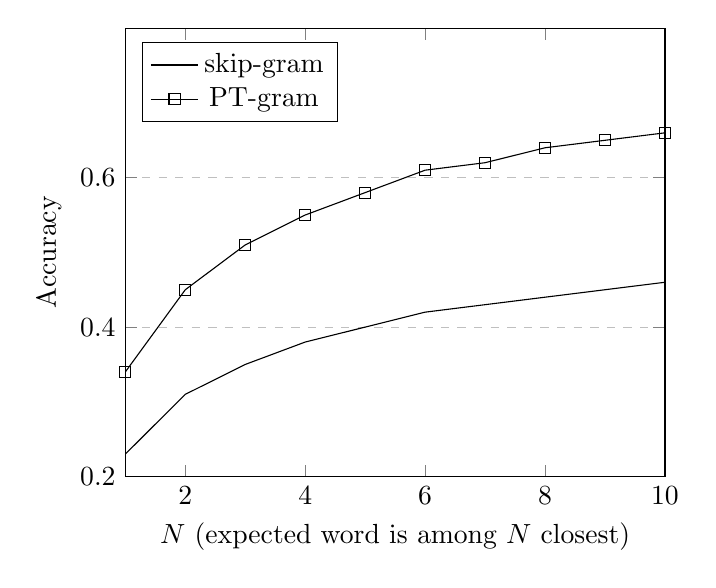
\begin{tikzpicture}
\begin{axis}[
    xlabel={$N$ (expected word is among $N$ closest)},
    ylabel={Accuracy},
    xmin=1, xmax=10,
    ymin=0.2, ymax=0.8,
    xtick={2,4,6,8,10},
    ytick={0.2,0.4,0.6},
    legend pos=north west,
    ymajorgrids=true,
    grid style=dashed,
]
\addplot[color=black]
    coordinates {(1,0.23)(2,0.31)(3,0.35)(4,0.38)(5,0.40)
                 (6,0.42)(7,0.43)(8,0.44)(9,0.45)(10,0.46)};
\addplot[color=black,mark=square]
    coordinates {(1,0.34)(2,0.45)(3,0.51)(4,0.55)(5,0.58)
                 (6,0.61)(7,0.62)(8,0.64)(9,0.65)(10,0.66)};
\legend{skip-gram,PT-gram}
\end{axis}
\end{tikzpicture}
\end{figure}
\end{center}

PT-gram model provides 45\% increase in the accuracy compared
to skip-gram trained on the same dataset with the same parameters.
Figure 1 presents the accuracy for both models depending on the
position of the expected word in the list sorted by the distance.
$N=1$ corresponds to the case when the expected word is the first in the
list, $N=2$ -- the word is among two closest, etc. Results for
commonly used $N=4$ (expected word is among four closest) are 0.36 for
skip-gram and 0.55 for PT-grams.

%1   0.23    0.34    1.43
%2   0.31    0.45    1.45
%3   0.35    0.51    1.46
%4   0.38    0.55    1.46
%5   0.40    0.58    1.46
%6   0.42    0.61    1.46
%7   0.43    0.62    1.45
%8   0.44    0.64    1.46
%9   0.45    0.65    1.46
%10  0.46    0.66    1.45

\section{Conclusion}

We've reviewed the modification of word2vec that is using parse tree
structure to form variable-size windows. The approach shows visible
increase in accuracy on analogy test. The increase comes at a cost --
the preprocessing of the original dataset is resource consuming and
may take longer than training the embedding model. Building parse trees
for a corpus of documents may also be sensitive to the quality of texts
-- grammar structure analysis might not tolerate errors, omissions, etc.

One of PT-gram model weaknesses is that the tree built for one sentence
doesn't take into account words in the surrounding sentences. The issue can
be addressed by using co-references between elements of different
sentences -- taking into account larger scale text structure may
provide additional increase in accuracy.


\bibliographystyle{unsrt}
\bibliography{ptgrams1}

\newpage
\section{Appendix. Parse tree and PT-grams: example}

Below is the parse tree for the following sentence:
\textit{According to one of the legends in the Acts, Thomas was at first reluctant to accept this mission, but the Lord appeared to him in a night vision and said, "Fear not, Thomas".}
\footnote{Wikipedia article about Thomas the Apostle}

\begin{scriptsize}
\tikzset{grow'=right}
\tikzset{every tree node/.style={anchor=base west}}
\Tree[.ROOT [.S [.S [.PP [.VBG According ] [.PP [.TO to ] [.NP [.NP [.CD one ] ] [.PP [.IN of ] [.NP [.NP [.DT the ] [.NNS legends ] ] [.PP [.IN in ] [.NP [.DT the ] [.NNS Acts ] ] ] ] ] ] ] ] [.NP [.NNP Thomas ] ] [.VP [.VBD was ] [.PP [.IN at ] [.NP [.NP [.JJ first ] ] [.ADJP [.JJ reluctant ] [.S [.VP [.TO to ] [.VP [.VB accept ] [.NP [.DT this ] [.NN mission ] ] ] ] ] ] ] ] ] ]  [.CC but ] [.S [.NP [.DT the ] [.NN Lord ] ] [.VP [.VP [.VBD appeared ] [.PP [.TO to ] [.NP [.PRP him ] ] ] [.PP [.IN in ] [.NP [.DT a ] [.NN night ] [.NN vision ] ] ] ] [.CC and ] [.VP [.VBD said ] [.S [.NP [.NP [.NN Fear ] [.RB not ] ] [.NP [.NNP Thomas ] ] ] ] ] ] ] ] ]
\end{scriptsize}

This tree structure corresponds to the following PT-grams
(with stop words removed and excluding one-word cases):

\begin{itemize}
\item legends Acts
\item one legends Acts
\item According one legends Acts
\item accept mission
\item reluctant accept mission
\item first reluctant accept mission 
\item According one legends Acts Thomas first reluctant accept mission 
\item appeared him night vision
\item Fear not Thomas
\item said Fear not Thomas
\item Lord appeared him night vision said Fear not Thomas
\end{itemize}


\end{document}


